\documentclass[11pt]{beamer}
\usetheme{Madrid}
\usecolortheme[named=blue]{structure}

% --- Custom Colors ---
\definecolor{navy}{HTML}{1A3F6E}
\definecolor{skyblue}{HTML}{87CEEB}   % light blue
\definecolor{lightblue}{HTML}{ADD8E6} % very soft blue
\setbeamercolor{title}{fg=white,bg=navy}
\setbeamercolor{frametitle}{fg=white,bg=navy}
\setbeamercolor{structure}{fg=navy}

\usepackage{graphicx}
\usepackage{booktabs}
\usepackage{caption}
\usepackage{tikz}
\usetikzlibrary{positioning}
\usepackage[table]{xcolor} 
\usepackage{booktabs}
\usepackage{float} % in preamble
\usepackage{colortbl} % for colored tables
\usepackage{xcolor}   % for color definitions
\usepackage{tcolorbox}

% --- Title Page Info ---
\title[Forecasting CNEPI]{Forecasting Sri Lanka’s Commodity Net
	Export Price Index Using ARIMA Models}
\author[Amali Rajapaksha]{Amali Rajapaksha \\ AS2022642}
\institute[Dept. of statistics]{Department of Statistics \\ University of Sri Jayewardenepura}
\date[Oct 2025]{October 2025}

\begin{document}
	
	%-----------------------------------------------------
	\begin{frame}
		\titlepage
		\vfill
		\tiny{Supervisor: Dr. Neluka Devpura \\ Department of Statistics }
	\end{frame}
	
	%-----------------------------------------------------
	\begin{frame}{Outline}
		\tableofcontents
	\end{frame}
	
	%-----------------------------------------------------
	\section{Introduction}
	\begin{frame}{Introduction}
		\begin{itemize}
			\item International trade
			mainly takes place in two directions, known as exports and imports.
			\vspace{0.3cm}
			\item The combined effect of exports and imports is measured by net exports, which is the
			difference between these two.
			\vspace{0.3cm}
			\item  For effectively monitoring and understanding these trade dynamics, it is important to depend on accurate and timely indicators.
			\vspace{0.3cm}
			\item \textbf{Commodity Net
			Export Price Index} is a important trade indicator.
		\end{itemize}
	\end{frame}
	
		%-----------------------------------------------------
	\section{Objectives}
	
	\begin{frame}{Objectives}
		\subsection*{Main Objective}
		\textbf{Main Objective}
		\begin{itemize}
			\item Forecast Sri Lanka’s Commodity Net Export Price Index using ARIMA models 
			by building a parsimonious statistical model.
		\end{itemize}
		
		\vspace{0.5cm}
		
		\subsection*{Specific Objective}
		\textbf{Specific Objective}
		\begin{itemize}
			\item Provide insights for policymakers, businesses, and researchers 
			regarding expected trends in trade and their implications for 
			economic stability.
		\end{itemize}
	\end{frame}
	
	
	%-----------------------------------------------------
	\section{Literature Review Summary}
	
	\begin{frame}{Literature Review Summary}
		\subsection*{In the world context}
		\textbf{In the world context}
		\begin{itemize}
			\item Researchers have forecasted:
			\begin{itemize}
				\item Imports and exports using various time series models
				\item Export price indices and survey-based indicators
			\end{itemize}
			\item But no net exports
		\end{itemize}
		
		\vspace{0.5cm}
		
		\subsection*{In Sri Lankan context}
		\textbf{In Sri Lankan context}
		\begin{itemize}
			\item Researchers have forecasted:
			\begin{itemize}
				\item Imports and exports using various time series models
			\end{itemize}
			\item But no net exports and any of the trade price indices
		\end{itemize}
\vspace{0.5cm}		
		
		\subsection*{The indicator that we studied in our research hasn’t been forecasted by any researcher so far.}
		\textbf{The indicator that we studied in our research
			hasn’t been forecasted by any researcher so far.}
		

	\end{frame}
	
	
	%-----------------------------------------------------
	\section{Data}
	\begin{frame}{Data}
		\begin{itemize}
			\item Source: International Monetary Fund (IMF)
			commodity terms of trade database
		
				
				\href{https://legacydata.imf.org/?sk=466fa59d-0ae3-40c9-b2a9-ac719d3a734e&hide_uv=1}{\textcolor{blue}{\underline{International Monetary Fund (IMF) – Legacy Data Portal}}}
			
			\vspace{0.5cm}
			\item Time duration : From 1980 January to 2025 March
			\vspace{0.5cm}
			\item Frequency: Monthly
			\vspace{0.5cm}
	
			\item Variable:  \textbf{Commodity Net Export Price Index}, Individual Commodities Weighted by
			Ratio of Net Exports to GDP
		\end{itemize}
		
	\end{frame}
	
    %-----------------------------------------------------
    
	\section{Methodology}
	\begin{frame}{Methodology}
		
			Methodology Steps:
			\begin{enumerate}
			\item  Stationarity testing 
			\item  Model identification via ACF/PACF
			\item  Model estimation 
			\item Forecast evaluation 
			\item Diagnostic checking
			\item Forecasting future values
		\end{enumerate}
		
		
	\end{frame}
	
	%-----------------------------------------------------
	\section{Model Development}
	\begin{frame}{Model Development}
		\begin{itemize}
			\item Split data set into two groups
		\end{itemize}
		\vspace{0.2cm}
		
		\centering
		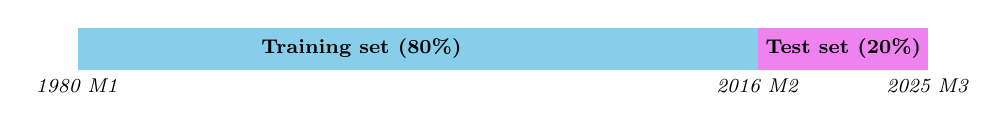
\begin{tikzpicture}[font=\footnotesize, scale=0.9, every node/.style={transform shape}]
			% Define colors
			\definecolor{trainblue}{HTML}{87CEEB}   % light sky blue
			\definecolor{testpink}{HTML}{EE82EE}    % soft magenta/pink
			
			% Draw training set (80%)
			\fill[trainblue] (0,0) rectangle (9.6,0.6);
			
			% Draw test set (20%)
			\fill[testpink] (9.6,0) rectangle (12,0.6);
			
			% Labels inside bars
			\node at (4,0.3) {\textbf{Training set (80\%)}};
			\node at (10.8,0.3) {\textbf{Test set (20\%)}};
			
			% Timeline years
			\node[below,font=\footnotesize] at (0,0) {\textit{1980 M1}};
			\node[below,font=\footnotesize] at (9.6,0) {\textit{2016 M2}};
			\node[below,font=\footnotesize] at (12,0) {\textit{2025 M3}};
		\end{tikzpicture}
		
		\vspace{0.9cm}
		
		\begin{itemize}
			\item No stationary (ADF test p = 0.3243)
		\end{itemize}
	
		\graphicspath{{C:/Users/MSI/OneDrive/Attachments/Pictures/}}
		\centering
		\begin{figure}
			\includegraphics[width=0.45\linewidth]{screenshot002.png}%
			\hfill
			\includegraphics[width=0.45\linewidth]{screenshot004.png}
			
		\end{figure}
		 \begin{itemize}
		 	\item No seasonal pattern
		 \end{itemize}
\end{frame}	 
	
\begin{frame}	

	
	\begin{itemize}
		\item Apply first differencing 
	\end{itemize}
		\vspace{0.5cm}
	\graphicspath{{C:/Users/MSI/OneDrive/Attachments/Pictures/}}
	\centering
		\includegraphics[width=0.45\linewidth]{screenshot006.png}%
		\hfill
		\includegraphics[width=0.45\linewidth]{screenshot007.png}
		
		\vspace{0.8cm} % optional small space
		
		% Tabular directly, no table float
		\begin{table}[H]
		\setlength{\tabcolsep}{6pt} 
		\renewcommand{\arraystretch}{1.3} 
		\begin{tabular}{l c c c c}
			\rowcolor{navy!80} 
			\textcolor{white}{\textbf{Test}} & 
			\textcolor{white}{\textbf{Data}} & 
			\textcolor{white}{\textbf{Test Statistic}} & 
			\textcolor{white}{\textbf{Lag Order}} & 
			\textcolor{white}{\textbf{p-value}} \\
			\rowcolor{blue!15} ADF Test Result & train\_ts\_diff & \textcolor{navy!20!black}{-7.6126} & 7 & \textcolor{red!70!black}{0.01} \\
		\end{tabular}
		{\footnotesize\textit{ADF test for differenced series}}
	\end{table}
	
\end{frame}	
	
	\begin{frame}
		\begin{itemize}
			\item ARIMA(1,1,1) selected as the initial candidate model
		\end{itemize}
		\vspace{0.5cm}
		\graphicspath{{C:/Users/MSI/OneDrive/Attachments/Pictures/}}
		\centering
		\includegraphics[width=0.48\linewidth]{screenshot007.png}%
		\hfill
		\includegraphics[width=0.48\linewidth]{screenshot011.png}
		
	\end{frame}
	
	
	%-----------------------------------------------------
	\section{Forecast Accuracy}
	\begin{frame}{Forecast Accuracy}
		\begin{itemize}
			\item ARIMA(2,1,3) selected as the best-performing model.
		\end{itemize}
	
		\definecolor{navyblue}{RGB}{5, 78, 100} % Custom navy blue
		\definecolor{lightblue}{RGB}{224, 235, 255} % Light background for alternate rows		
				\begin{table}[h!]
					\centering
					\footnotesize
					\renewcommand{\arraystretch}{0.9} % Row height
					\setlength{\tabcolsep}{6pt} % Column separation
					\rowcolors{2}{white}{lightblue} % Alternating row colors
					
					\begin{tabular}{l c c c c c c}
						\hline
						\rowcolor{navyblue}
						\color{white}\textbf{ARIMA} & 
						\color{white}\textbf{AIC} & 
						\color{white}\textbf{BIC} & 
						\multicolumn{4}{c}{\color{white}\textbf{Testing Set}} \\ 
						\cline{4-7}
						\rowcolor{navyblue}
						\color{white} & \color{white} & \color{white} & 
						\color{white}\textbf{RMSE} & 
						\color{white}\textbf{MAE} & 
						\color{white}\textbf{MAPE} & 
						\color{white}\textbf{MASE} \\
						\hline
						(1,1,1) & 425.39 & 441.67 & 3.6540 & 3.2925 & 3.296 & 2.8390 \\
						(0,1,1) & 424.27\textcolor{red}{*} & 436.48\textcolor{red}{*} & 3.6289 & 3.2657 & 3.269 & 2.8159 \\
						(1,1,0) & 427.50 & 439.71 & 3.6310 & 3.2689 & 3.272 & 2.8186 \\
						(0,1,0) & 447.85 & 455.99 & 3.7629 & 3.4089 & 3.412 & 2.9394 \\
						(2,1,2) & 428.98 & 453.40 & 3.6156 & 3.2572 & 3.261 & 2.8086 \\
						(2,1,1) & 427.06 & 447.42 & 3.6549 & 3.2936 & 3.297 & 2.8400 \\
						(1,1,2) & 426.85 & 447.20 & 3.6457 & 3.2833 & 3.287 & 2.8311 \\
						(2,1,0) & 426.23 & 442.52 & 3.6345 & 3.2717 & 3.275 & 2.8211 \\
						(0,1,2) & 425.54 & 441.82 & 3.6463 & 3.2845 & 3.288 & 2.8321 \\
						(1,1,3) & 428.78 & 453.20 & 3.6410 & 3.2793 & 3.283 & 2.8277 \\
						(3,1,1) & 428.71 & 453.13 & 3.6415 & 3.2792 & 3.283 & 2.8276 \\
						(3,1,2) & 428.68 & 457.17 & 2.6689 & 2.2918 & 2.297 & 1.9762 \\
						(2,1,3) & 428.24 & 456.74 & 2.3036\textcolor{red}{*} & 2.0122\textcolor{red}{*} & 2.0156\textcolor{red}{*} & 1.7351\textcolor{red}{*} \\
						(3,1,3) & 430.67 & 463.24 & 2.6888 & 2.3091 & 2.3148 & 1.9911 \\
						(3,1,0) & 428.07 & 448.42 & 3.6427 & 3.2805 & 3.2838 & 2.8286 \\
						\hline
					\end{tabular}
					
				\end{table}
		
		
	\end{frame}
	
	%-----------------------------------------------------
	\section{Model Diagonestic}
	\begin{frame}{Model Diagonestic}
		\begin{itemize}
			\item Residuals are independent (Box–Ljung p = 0.9905).
		\end{itemize}
		\graphicspath{{C:/Users/MSI/OneDrive/Attachments/Pictures/}}
		\centering
		\includegraphics[width=0.40\linewidth]{screenshot013.png}%
		\hfill
		\includegraphics[width=0.40\linewidth]{screenshot014.png}
		
		\vspace{-0.1cm}
		\begin{itemize}
			\item Residuals satisfies the zeroth mean and the constant variance
		\end{itemize}
	
		\vspace{-0.1cm}
			\graphicspath{{C:/Users/MSI/OneDrive/Attachments/Pictures/}}
		\includegraphics[width=0.41\linewidth]{screenshot015.png}
		
		\begin{itemize}
			\item Residuals are not normal (Shapiro-Wilk Test p = 0.0012)
		\end{itemize}
	\end{frame}
	
	%-----------------------------------------------------
	\section{Results and Forecasts}
	\begin{frame}{Results and Forecasts}
		
		
		\definecolor{navyblue}{RGB}{0,48,80}
		\setbeamercolor{block title}{bg=navyblue, fg=white}
		\setbeamercolor{block body}{bg=navyblue!10, fg=navyblue}
		
			\begin{block}{Final model equation}
				\[
				\resizebox{1.0\textwidth}{!}{$
					Y_t = -0.0022 + B\,Y_{t} + 0.1130(1-B)B\,Y_{t} + 0.8485(1-B)B^{2}Y_{t}
					+ 0.1279\,B\,Z_{t} - 0.9217\,B^2\,Z_{t} - 0.2062\,B^3\,Z_{t} + Z_t
					$}
				\]
			\end{block}
			
			\scriptsize\textcolor{navyblue}{
				Note: \(B\) denotes the backshift operator where \(B\,Y_t = Y_{t-1}\).
			}
			\vspace{0.3cm}
			\begin{itemize}
				\item Forecasted CNEPI from 2025 April to 2026 March
			\end{itemize}
			
			\begin{table}[h!]
				\centering
				\renewcommand{\arraystretch}{0.9} % Row height
				\setlength{\tabcolsep}{10pt} % Column spacing
				
				% ----- Table caption -----
				\label{tab:forecast_values}
				
				% ----- Table body -----
				\rowcolors{2}{navyblue!5}{white} % Alternate row colors
				
				\begin{tabular}{>{\bfseries\color{navyblue}}l >{\color{navyblue}}l >{\color{black}}r}
					\hline
					\rowcolor{navyblue!25}
					\textbf{Year} & \textbf{Month} & \textbf{Forecasted Value} \\
					\hline
					2025 & April      & 100.8114 \\
					2025 & May        & 100.8102 \\
					2025 & June       & 100.8325 \\
					2025 & July       & 100.8339 \\
					2025 & August     & 100.8529 \\
					2025 & September  & 100.8561 \\
					2025 & October    & 100.8725 \\
					2025 & November   & 100.8770 \\
					2025 & December   & 100.8913 \\
					2026 & January    & 100.8967 \\
					2026 & February   & 100.9094 \\
					2026 & March      & 100.9153 \\
					\hline
				\end{tabular}
			\end{table}
			
	\end{frame}
	
	\begin{frame}
		\graphicspath{{C:/Users/MSI/OneDrive/Attachments/Pictures/}}
		\includegraphics[width=1.0\linewidth]{screenshot016.png}
	\end{frame}
	
	%-----------------------------------------------------
	
	\section{Conclusion}
	\begin{frame}{Conclusion}
		\begin{itemize}
			\item ARIMA(2,1,3) effectively forecasts Sri Lanka’s CNEPI.
			\end{itemize}	
			\vspace{0.5cm}
				\begin{itemize}
			\item The forecasts suggest a gradual
			upward trend, with values rising from 100.81 in April 2025 to 100.92 by March 2026. This
			indicates a modest recovery and stabilization of Sri Lanka’s net export competitiveness
			soon.
				\end{itemize}
			\vspace{0.5cm}
				\begin{itemize}
			\item Export businesses
			can use these forecasts to make better plans since the increasing trend shows Sri Lanka’s
			products are becoming more competitive in world markets.
		\end{itemize}
		
	\end{frame}
	
	%-----------------------------------------------------
	\section{Limitations and Future Research }
	\begin{frame}{Limitations and Future Research}
		\begin{itemize}
			\item The index used in the study is only for commodities and does not include growing shares
			of the services provided in Sri Lanka’s trade.  These should be added to the future indices.
		\end{itemize}
		\vspace{0.4cm}
		
		\begin{itemize}
			\item ARIMA rely only on the past values of the index.The effect of other exogenous factors such as exchange rates, interest rate can be included in the forecasting models. 
		\end{itemize}
		\vspace{0.4cm}
		
		\begin{itemize}
			\item The machine learning approaches can be considered in the future.
		\end{itemize}
		
	\end{frame}
	
	%-----------------------------------------------------
	\begin{frame}{References}
		\begin{enumerate}
			\item Hyndman, R.J. \& Athanasopoulos, G., 2021. Forecasting: principles and practice.
			3rd ed. Melbourne: OTexts.
			\vspace{0.5cm} 
			\item Gruss, B. \& Kebhaj, S., 2019. Commodity Terms of Trade: A New Database. IMF Working Paper No. 19/21. Washington, D.C.: International Monetary Fund.
			\vspace{0.5cm}
			\item Dridi, J. and Zieschang, K., 2004. Export and import price indices. IMF Staff
			Papers, 51(1), pp.157-194.
		\end{enumerate}
	\end{frame}
	
	%-----------------------------------------------------
	\begin{frame}{Thank You}
		\centering
		\Large \textbf{Thank You!} \\
		\vspace{0.3cm}
		\normalsize Questions and comments are welcome. \\
		\vfill
		\tiny{Prepared by Amali Rajapaksha — Department of Statistics, University of Sri Jayewardenepura}
	\end{frame}
	
\end{document}
